\begin{frame}{Physical state}
\centering
\hspace{-1cm}
\begin{tikzpicture}[scale=1.15]
	\def\hist{2}
	\def\histext{1}
	\def\pub{3}
	\def\priv{2.8}
	
	\only<1->{
		\draw[step=1cm, gray, thin] (0, 0) grid (\hist + \pub + \priv, 1) ;
		\draw[decorate, decoration={brace, amplitude=5pt}] (-0.2, 0) -- (-0.2, 1) node [midway, xshift=-7mm] {data} ;
	}
	
	\only<2->{
		\draw[very thick] (\hist, 0) -- (\hist, 1) node[label=above:front] {} ;
	}
	
	\only<4->{
		\draw[very thick] (\hist + \pub, 0) -- (\hist + \pub, 1) node[label=above:back] {} ;
	}
	
	\only<5->{
		\fill[red, opacity=0.2] (\hist + \pub, 0) rectangle (\hist + \pub + \priv, 1) ;
		\draw[decorate, decoration={brace, amplitude=5pt}] (\hist + \pub + \priv, -0.2) -- (\hist + \pub, -0.2) node [midway, yshift=-5mm] {priv} ;
	}
	
	\only<6->{
		\fill[green, opacity=0.2] (\hist, 0) rectangle (\hist + \pub, 1) ;
		\draw[decorate, decoration={brace, amplitude=5pt}] (\hist + \pub, -0.2) -- (\hist, -0.2) node [midway, yshift=-5mm] {pub} ;
	}
	\only<7->{
		\fill[blue, opacity=0.2] (0,0) rectangle (\hist, 1) ;
		\draw[decorate, decoration={brace, amplitude=5pt}] (\hist, -0.2) -- (0, -0.2) node [midway, yshift=-5mm] {hist} ;
	}
		
	\only<9->{
		\fill[blue, opacity=0.2] (\hist,0) rectangle (\hist + \histext, 1) ;
		\draw[decorate, decoration={brace, amplitude=5pt}] (\hist + \histext, -1) -- (0, -1) node [midway, yshift=-5mm] {hist\textsubscript{+}} ;
	}
	
	\only<10->{
		\draw[thick, ->, blue] (\hist, 0.5) -- (\hist + 1, 0.5) node[label=below left:{\footnotesize\texttt{steal}}] {} ;
		\draw[thick, ->, teal] (\hist + \pub, 0.5) -- (\hist + \pub - 1, 0.5) node[label=below right:{\footnotesize\texttt{pop}}] {} ;
		\draw[thick, ->, red] (\hist + \pub, 0.5) -- (\hist + \pub + 1, 0.5) node[label=below left:{\footnotesize\texttt{push}}] {} ;
	}
\end{tikzpicture}
\vfill
\begin{itemize}
	\item[data:]<1-> infinite array storing all values
	\item[front:]<2-> \emph{monotone} index for thieves' end
	\item[back:]<4-> index for owner's end
\end{itemize}
\begin{itemize}
	\item[priv:]<5-> list of private values (controlled by owner)
	\item[pub:]<6-> list of public values (= model)
	\item[hist:]<7-> \emph{monotone} list of history values
	\item[hist\textsubscript{+}:]<9-> \emph{monotone} list of extended history values
\end{itemize}
\begin{overbox}<3>
	\begin{mathpar}
		\inferrule*[lab=ChaselevFrontValid]
			{
				\iGhost{\gamma\mathrm{.front}}{\iAuth{front_1}}
			\and
				\iGhost{\gamma\mathrm{.front}}{\iFrag{front_2}}
			}{
				front2 \leq front1
			}
		\and
		\inferrule*[lab=ChaselevFrontUpdate]
			{
				front \leq front'
			\and
				\iGhost{\gamma\mathrm{.front}}{\iAuth{front}}
			}{
				\iGhost{\gamma\mathrm{.front}}{\iAuth{front'}}
			}
		\and
		\inferrule*[lab=ChaselevFrontFragGet]
			{
				\iGhost{\gamma\mathrm{.front}}{\iAuth{front}}
			}{
				\iGhost{\gamma\mathrm{.front}}{\iFrag{front}}
			}
	\end{mathpar}
\end{overbox}
\begin{overbox}<8>
	\begin{mathpar}
		\inferrule*[lab=ChaselevHistValid]
			{
				\iGhost{\gamma\mathrm{.hist}}{\iAuth{hist_1}}
			\and
				\iGhost{\gamma\mathrm{.hist}}{\iFrag{hist_2}}
			}{
				hist_2 \sqsubseteq_\mathrm{prefix} hist_1
			}
		\and
		\inferrule*[lab=ChaselevHistUpdate]
			{
				\iGhost{\gamma\mathrm{.hist}}{\iAuth{hist}}
			}{
				\iGhost{\gamma\mathrm{.hist}}{\iAuth{(hist \mdoubleplus [v])}}
			}
		\and
		\inferrule*[lab=ChaselevHistFragGet]
			{
				\iGhost{\gamma\mathrm{.hist}}{\iAuth{hist}}
			}{
				\iGhost{\gamma\mathrm{.hist}}{\iFrag{hist}}
			}
	\end{mathpar}
\end{overbox}
\end{frame}

% ---------------------------------------------------------

\begin{frame}{Logical state}
\centering
\begin{tikzpicture}
	\def\width{4cm}
	\def\height{2cm}
	
	\only<1->{
		\node[align=center] (s1) {
			\ding{172} empty \\
			\begin{tikzpicture}[scale=0.5]
				\def\hist{2}
				\def\priv{2.8}
		
				\draw[step=1cm, gray, thin] (0, 0) grid (\hist + \priv, 1) ;
				
				\fill[blue, opacity=0.2] (0, 0) rectangle (\hist, 1) ;
				\draw[very thick] (\hist, 1) -- (\hist, 0) node[yshift=2mm, label=below:{\tiny front = back}] {} ;
				\fill[red, opacity=0.2] (\hist, 0) rectangle (\hist + \priv, 1) ;
			\end{tikzpicture}
	   } ;
	   
	   \node[align=center] (s2) [right=\width of s1] {
	   		\ding{173} non-empty \\
			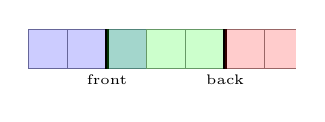
\begin{tikzpicture}[scale=0.5]
				\def\hist{2}
				\def\histext{1}
				\def\pub{3}
				\def\priv{1.8}
		
				\draw[step=1cm, gray, thin] (0, 0) grid (\hist + \pub + \priv, 1) ;
				
				\fill[blue, opacity=0.2] (0, 0) rectangle (\hist + \histext, 1) ;
				\draw[very thick] (\hist, 1) -- (\hist, 0) node[yshift=2mm, label=below:{\tiny front}] {} ;
				\fill[green, opacity=0.2] (\hist, 0) rectangle (\hist + \pub, 1) ;
				\draw[very thick] (\hist + \pub, 1) -- (\hist + \pub, 0) node[yshift=2mm, label=below:{\tiny back}] {} ;
				\fill[red, opacity=0.2] (\hist + \pub, 0) rectangle (\hist + \pub + \priv, 1) ;
			\end{tikzpicture}
	   } ;
   }
   
   \only<3->{
	   \node[align=center] (s3) [below=\height of s2] {
	   		\ding{174} emptyish \\
			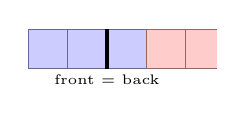
\begin{tikzpicture}[scale=0.5]
				\def\hist{2}
				\def\histext{1}
				\def\priv{2.8}
		
				\draw[step=1cm, gray, thin] (0, 0) grid (\hist + \priv, 1) ;
				
				\fill[blue, opacity=0.2] (0, 0) rectangle (\hist + \histext, 1) ;
				\draw[very thick] (\hist, 1) -- (\hist, 0) node[yshift=2mm, label=below:{\tiny front = back}] {} ;
				\fill[red, opacity=0.2] (\hist + \histext, 0) rectangle (\hist + \priv, 1) ;
			\end{tikzpicture}
	   } ;
	   \node[align=center] (s4) [below=\height of s1] {
	   	\ding{175} super empty \\
			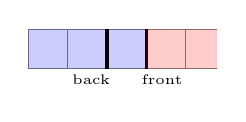
\begin{tikzpicture}[scale=0.5]
				\def\hist{2}
				\def\histext{1}
				\def\priv{2.8}
		
				\draw[step=1cm, gray, thin] (0, 0) grid (\hist + \priv, 1) ;
				
				\fill[blue, opacity=0.2] (0, 0) rectangle (\hist + \histext, 1) ;
				\draw[very thick] (\hist, 1) -- (\hist, 0) node[xshift=-2mm, yshift=2mm, label=below:{\tiny back}] {} ;
				\draw[very thick] (\hist + \histext, 1) -- (\hist + \histext, 0) node[xshift=2mm, yshift=2mm, label=below:{\tiny front}] {} ;
				\fill[red, opacity=0.2] (\hist + \histext, 0) rectangle (\hist + \priv, 1) ;
			\end{tikzpicture}
	   } ;
   }
   
   \only<2->{
	   \draw[thick, ->] (s1) to[bend left] node[above] {push} (s2) ;
	   \draw[thick, ->] (s2) to[bend left] node[below] {steal} (s1) ;
	   \draw[thick, ->] (s2) to[looseness=3, out=135, in=45] node[above] {push, pop, steal} (s2) ;
   }
   \only<4->{
	   \draw[thick, ->] (s2) to[bend left] node[right] {pop} (s3) ;
	   \draw[thick, ->] (s3) to[bend left] node[below] {pop, steal} (s4) ;
	   \draw[thick, ->] (s4) to[bend left] node[left] {pop} (s1) ;
   }
   \only<5->{
   		\draw[thick, ->] (s1) to[bend left] node[right] {pop} (s4) ;
   }
\end{tikzpicture}
\end{frame}